% !TeX spellcheck = en_US 
\chapter{System Requirements} \label{Requirements}
%\section{Description of requirements} 

\section{Motivation} In the end of most kinds of investigation there needs to be an examiner, an auditor or generally an intelligent person, who would understand what happened in the case. 
Their aim is to ascertain who is responsible for it. In this situation the examiner usually already has some outputs from some software, for example from software described in \ref{Analysis}. However, the situation may be quite complex and the examiner may be using more than one piece of software in this stage. The inspected period of time can be also relatively long. Altogether it can cause difficulties, make the task harder and as a result prolong the time of investigation. Our application should help forensic auditors, to see what was happening in the case during the examined period of time. This application should provide the possibility to see the big picture and so help with the investigation.

The end of the investigation is also specific in the aspect that there are not so many subjects that play the main role in the case. Usually the most important participants are already known. This application is ideal for a situation where there are approximately  five to fifteen subjects. It is possible to process the database where there is much higher number of subjects. Examines, e.g. users can adjust which subjects they want to track. This application can be useful when a fraud is being uncovered, when some of the subjects pursue a corruption practice and also in other similar scenarios of a similar kind. 

The system should allow the auditor to replay and visually show what was happening during the investigated period. 

\section{Graphical User Interface}

We have decided that the scheme of graphical user interface of our program will be as shown in figure \ref{predstava}. The main and most important part of the area of the application should be the middle frame. This frame should contain one dot for each subject of our case. These dots will be in a circle by default, however, the user should be able to move them freely in the frame area. The visualization should also be later replayed in this place. This visualization is the bigger picture that the application should provide to the user. 

As shown in figure \ref{predstava} there should be a time axis under this panel with a slider and play/stop button. After clicking the play/stop button, the main action of this application should start. In the middle frame the dots representing the subjects should each display an activity every time the subject is involved in some event. The application should process activities which are mentioned and explained later on.


\begin{figure}[h]
	\begin{center} 
	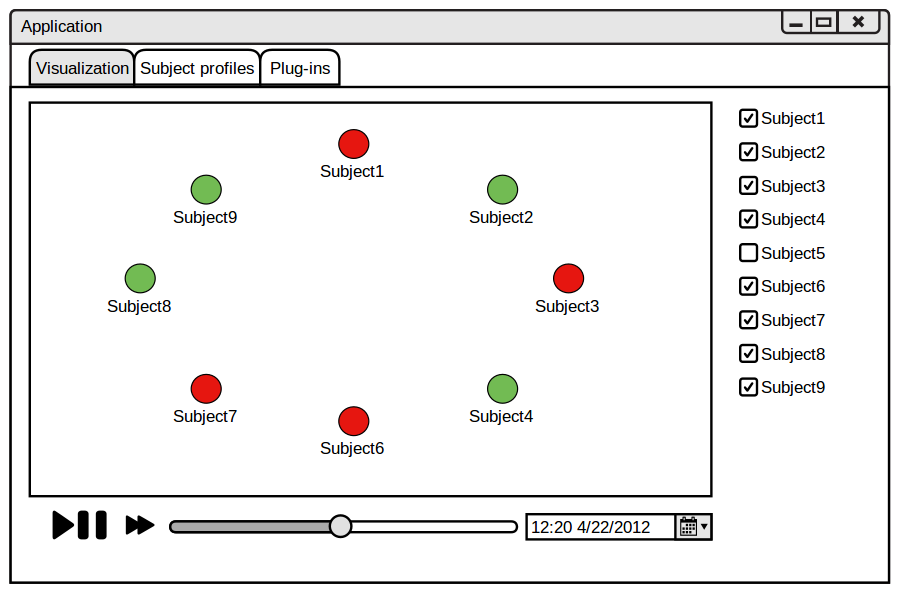
\includegraphics[width=1.0\textwidth]{./img/GUI/visualization.png}
	\end{center}
	\caption{GUI Scheme}\label{predstava}
\end{figure}

\section {Activities of the application} %<Files/Displayer-inside.jpg> // It should look like this, but the picture needs to have higher level, obviously
%\todo{TODO: pridat UML diagram akci}
%\section{Working with the application}
\paragraph{Selecting subjects}
Users should be able to select whatever subset of actions and subjects they want to replay in the animation of the case. After uploading the data, the application should generate names of all subjects and next to each one of them a check-box widget. Users should have the possibility to choose from them. Generally it would also be good to provide a possibility to choose a subset of all events directly from our database using a SQL query.

\paragraph{Adjusting the time period}
Under the animation frame there should be a scroll bar and a field indicating the corresponding time and date. Users should be able to move the scroll the bar below the animation frame manually and this way to travel in investigated period of time. At each point the corresponding scene should appear in the animation frame. The time should also be adjustable manually in the field that indicates corresponding time and date. After clicking the Play/Stop button replaying the visualization from this time further should start. 

\paragraph{Visualization}
After clicking on the button play/stop the animation of the scene should start replaying. The program will go through the database of events that the subjects did and for each event a spot representing the subject will change its color for a constant time period. If user stops (pauses) this playback and then starts it again the animation should continue from where it stopped. There should be a possibility to adjust the speed of replaying the case. 

\paragraph{Modes of replaying}
The application should provide two modes of replaying. First mode should be replaying according to the real time. Between every two events there should be the same proportion of time with regard to the time in reality. The purpose of this mode is to give the forensic auditor the idea of the time flow in the case. Second mode would serve as a quick replay of events. The period of time that has passed between every two events should be represented by a constant period of time in the visualization. The speed of time flow while replaying should be adjustable in both modes.

\paragraph{Subject activities}
The application should distinguish between several types of subject activities as shown in following overview.

%Activity | Example | Action
\begin{tabularx}{\textwidth}{l X}
Activity: & There is currently no Event involving this Subject.\\
Action: & The color of the dot representing the subject is red (Fig.\ref{subj_doing_nothing})\\
& 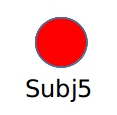
\includegraphics[scale=0.3]{./img/visualization/subj_doing_nothing.png}\label{subj_doing_nothing}\\
\end{tabularx}\\

\begin{tabularx}{\textwidth}{l X}
%\hline
Activity: & Subject is doing something e.g. subject is causing an event\\
Example: & Subject4 is buying a new yacht. \\
Action: & The color of the dot representing the subject changes from red (no action) to green (indicating activity). After a globally adjustable time period the event the color of the dot changes back to red. If we have details about this event a small icon appears above the dot  revealing details of the event.\\ 
& 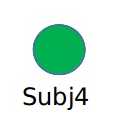
\includegraphics[scale=0.3]{./img/visualization/subj_doing_sth.png}\\
\end{tabularx}\\

%\begin{figure}[h]
%	\begin{center} \label{subj_doing_sth}
%	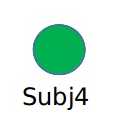
\includegraphics[]{./img/visualization/subj_doing_sth.png}
%	\end{center}
%	\caption{Activity of a subject}
%\end{figure}


\begin{tabularx}{\textwidth}{l X}
%\hline
Activity: & Subject is causing an event related to another subject. \\
Example: & Subject1 transfers some amount of money to Subject2's bank account.\\
Action: & The dot of the active subject changes color to green and a arrow from the active subject to the related one appears. After a globally adjustable time period the arrow disappears and the color of the dot changes back to red. If we have details about this event a small icon appears above the arrow. After clicking on it the icon reveals details of the event. \\
& 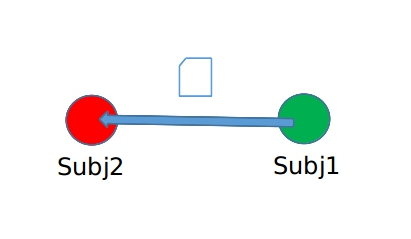
\includegraphics[scale=0.3]{./img/visualization/subj_sending_msg.png}\\


\end{tabularx}\\
\begin{tabularx}{\textwidth}{l X}
%\hline
Activity: & Several subjects are part of a event together. \\
Example: & Subject3, Subject6 and Subject7 have a business meeting together.\\
Action: & All dots representing corresponding subjects change color and a line connecting them together appears. After a globally adjustable time period all the dots are in default state (red color, no linking). If we have details about this event a small icon appears above the arrow. After clicking on it the icon reveals details of the event.\\
& 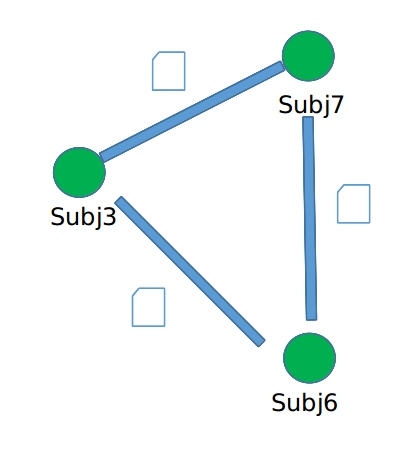
\includegraphics[scale=0.3]{./img/visualization/subjects_together.png}\\

\end{tabularx}



\section{Data}
The application should process data from very different sources. Since the application shall be used in last stages of forensic audit we expect that the data might be pre-selected by some quantitative or analytical software. Even though the application should not be limited by the amount of data, average usage is expected to work with the order of hundreds of events. Visualization of more events may not have the effect to help understand the situation. However, the application should be able to hold much more data in the database so that the forensic auditor could select form them.

Since there are many sources of data of different structure in forensic audit, our application is expected work as a superstructure with the purpose of the data projection only. The application should use data inserted to the application by various plug-ins. These plug-ins should transform the structure of data stored in the source (for example, instant messenger, email, accounting system, data from social networks etc.) to the data format used in our application. This two-layer division is chosen as it is easily expandable and universal. This project describes a standard interface for communication with these plug-ins.


Even though the implementation is not part of this project and the aim of this project is only to design the application, the design should be precise enough to make the implementation easy. 


\section{Example case}

The action of this application may be represented in following example case. Let us presume there is a company named "XYZ" where some money is missing. However, we are aware of those specific employees, of that certain enterprise, who have direct access to the company accounts. We also know the certain managers that are responsible for the company investments. Moreover, there are business partners of the company and also some regular employees such as workers. This case of money being disappeared has occurred during the period of 6 months. 

Forensic auditors receive the data from internal email, IM, telephone communication, from internal accounting system and is aware of the business operations of the company. They have also investigated information on the Internet on social sites. After accumulating all the data they use some analytical or quantitative software \ref{qSW} to discover the abnormalities in the accounting evidence. The rec SW recognize various connections between some of the subjects (common after work activities, common interests etc.). They have enough input, but still they need to find out what exactly happened. 

Forensic auditors decide to make use of our application for the investigative procedure. Firstly, they load all the outputs to the application and then they replay the events that happened during the last 6 months. Our system gives them an opportunity to deselect some subjects that seem to be irrelevant. They can also select the set of information for replaying via SQL query, i.e. the forensic auditor may arbitrarily replay those specific events that they demand. 




%To be able to design a new application 
%
%we need to make a series of decision and answer number of questions going from the most general to the most concrete. 
%Decisions and answers of the questions from the most general to the most concrete 
%
%All the decisions needed to be made to design the application are stated in the 


%\paragraph{Data format requirement} Our data will contain information of following structure: 
%every record of an action will contain ID of an record, name of the active subject, name(s) of 
%passive subject(s), the time of the action, and the record of remarks including details about 
%the action. These records will be stored in a database. We will be able to access all the 
%information. 
%
%
%\paragraph{Estimating the amount of data} We expect that our application will be used in final 
%stages of forensic audit, when we know the key period and only a few subjects remain. We expect 
%that we will be working with an order of hundreds of entries.






%\section{Working with the application}
%After uploading the data, the application should generate names of all subjects and for each one of them a check-box widget. This way users can select which subject they want in the animation of the case and which they want to displace in the next animation. 
%
%Below the animation frame there should be a scroll bar and a field indicating the corresponding time and date. Users should be able to move the scroll bar below the animation frame manually and this way to travel in investigated period of time. In each point a corresponding scene should appear in the animation frame. The time should also be adjustable manually in the field that indicates corresponding time and date. 
%
%User of this application should also have the possibility to select a subset of all events in the database using a SQL query. 
%
%After clicking on the button play/stop the animation of the scene should start replaying.The program will go through the database of events that the subjects did and for each event a spot representing the subject will change its color for an adjustable period.  If user stops (pauses) this playback and then starts it again the animation should continue. There should be a possibility to adjust the speed of replaying the case. 

%\subsection{GUI requirements} 
%We have decided that the user interface of our program will look 
%as follows. The main part of the area will be the middle panel. We want this panel to contain 
%one spot for each subject of our case. These spots will be in a circle by default. This will be 
%the part of visualization that will help understand the sequence of events. 
%
%There will be a time axis under this panel with a slider and play and stop buttons. After 
%clicking the play button, the main action of this application will start. The program will go 
%through the database of events that the subjects did and for each event a spot representing the 
%subject will change its color for an adjustable period. 

%\todo{TODO: pridat obrazek priblizneho vysledku}


